\documentclass[10pt,utf8x]{beamer}

\usepackage{header}

\begin{document}
\setbeamercovered{transparent}

%-------------------------------------------------------------------------------
\begin{frame}
    \makemytitle
\end{frame}
%-------------------------------------------------------------------------------

%-------------------------------------------------------------------------------
\begin{frame}{Theory}
  \begin{block}{test}
      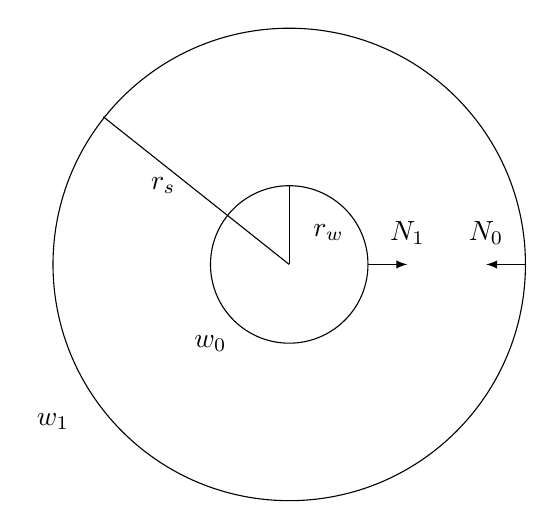
\begin{tikzpicture}
          \draw  (0,0) node (v1) {} ellipse (3 and 3);
          \draw  (0,0) ellipse (1 and 1);
          \draw [-latex](1,0) -- (1.5,0);
          \draw [-latex](3,0) -- (2.5,0);
          \draw (0,0) -- (-2.3611,1.8752);
          \draw (0,0) -- (0,1);
          \node at (-1,-1) {$w_0$};
          \node at (-3,-2) {$w_1$};
          \node at (-1.6,1) {$r_s$};
          \node at (0.5,0.4) {$r_w$};
          \node at (1.5,0.4) {$N_1$};
          \node at (2.5,0.4) {$N_0$};
      \end{tikzpicture}
  \end{block}
\end{frame}
%-------------------------------------------------------------------------------

%-------------------------------------------------------------------------------
\begin{frame}[allowframebreaks]{References}
  \vspace{-0.05\textheight}
  \scriptsize
  \bibliographystyle{apalike}
  \bibliography{seme2014_axessim}
\end{frame}
%-------------------------------------------------------------------------------

%%% Local Variables:
%%% coding: utf-8
%%% mode: latex
%%% TeX-PDF-mode: t
%%% TeX-parse-self: t
%%% TeX-auto-save: t
%%% x-symbol-8bits: nil
%%% TeX-auto-regexp-list: TeX-auto-full-regexp-list
%%% TeX-master: t
%%% ispell-local-dictionary: "american"
%%% End:

\end{document}
